
%
% foundations - spatial data
%

\section{Spatial data}

A central aspect in web mapping is dealing with spatial data. Decisions on how to structure and store spatial data highly influence the computation tasks that may be performed on such data. This mainly depends on the type of spatial data, where points are the most basic of all. Depending on the use case, different types of data are to be represented and stored: points, lines, rectangles, regions, surfaces and/or volumes. While most of the discussed concepts may be extended or generalized for processing more complex types of data, this is out of scope for this thesis. Instead, we focus on points as the most common type of spatial data~\cite{Samet90spatialdata}.

One fundamental way to store spatial data is the quadtree, a hierarchical data structure based on recursive decomposition of space. Hanan Samet attributes the history of quadtrees (and octrees which are their 3-dimensional extension) to Dijkstra, who invented a one-level decomposition of a matrix into square blocks. Morton then applied this technique to creating a spatial index (z-order). We will first discuss space orders \& decomposition and then put those into context when outlining the basics of the quadtree.


\subsection{Space order methods}
\label{chapter:space-order}

In order to store multi-dimensional, spatial data in a sequential storage like computer memory, the data needs to be serialized. Consider a pixel image as an example. Its 2-dimensional pixel values are positioned in planar space. In order to store the image, those pixels have to be processed in a predefined order, such that they can be serialized into a 1-dimensional array of memory units.

The traditional order for storing a raster of image data was row by row. The row order sequentially processes the raster row by row from left to right, starting at the top left corner. In contrast, the row-prime order switches the horizontal processing direction at the end of each row. This leads to a higher locality as it has the property of always moving to a 4-neighbor~\cite{Goodchild83raster}.

Besides the discussed row orders, additional space-ordering methods have been developed to serve different purposes. The Morton and Peano-Hilbert orders both visit entire sub quadrants first before before exiting them. The Morton order is easier to compute, because the position (key) of each element in the ordering can be determined by interleaving the bits of the x and y coordinates of that element. One disadvantage of the Morton order are the gaps: the longest move in a raster of $2^n$ by $2^n$ is one column and $2^n - 1$ rows (or vice versa). A better locality is offered by the Hilbert-Peano order which always has the property of moving to a 4-neighbor. This advantage on the other hand has the cost of a more complex definition. Calculating keys for the Hilbert-Peano order is more difficult. The higher complexity of the Hilbert-Peano obviously shows that its recursion is harder to define as well. Figure~\ref{fig:space-orders} illustrates these fundamental space orders with two further ones that allow for ordering unbounded space in two (Cantor-diagonal order) or four directions (spiral order)~\cite{Samet90spatialdata}.

\begin{figure}[h]
  \begin{center}
    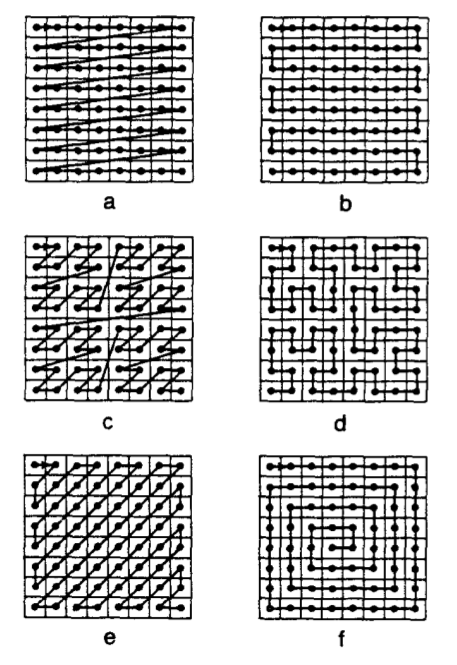
\includegraphics[width=0.5\textwidth]{figures/space_orders.png}
    \label{fig:space-orders}
    \caption{The result of applying a number of different space-ordering methods to an $8 \times 8$ image whose first element is in the upper left corner of the image: (a) row order, (b) row-prime order, (c) Morton order, (d) Peano-Hilbert order, (e) Cantor-diagonal order, (f) spiral order~\cite[p 14]{Samet90spatialdata}.}
  \end{center}
\end{figure}

The fact that the Hilbert-Peano order has the property of always moving to a 4-neighbor shouldn't be misinterpreted as still there are gaps. ``A bijective mapping from multidensional data to one dimension cannot be done the way that in any case nearby multidimensional points are also close together in one dimension~\cite{Tropf81multidimensional}''. Figure~\ref{fig:space-orders} clearly shows what Samet describes as ``both the Morton and Peano-Hilbert order exhaust a quadrant or subquadrant of a square image before exiting it~\cite{Samet90spatialdata}''. This means that the orders maintain locality for those quadrants based on the hierarchy, but the edges are still disconnected. The same issue will be dealt with further in Geohash (TODO Geohash).


\subsection{Space decomposition methods}

By definition, space decomposition methods partition space in a way so that,
\begin{itemize}
\item partitions are infinitely repetitive patterns for images of any size,
\item partitions are infinitely decomposable to generate finer sub-partitions of higher resolution.~\cite{Samet90spatialdata}
\end{itemize}

Various space decomposition methods exist. They can be classified depending on the shapes that are used for the partitioning patterns. Polygonal shapes are computationally simpler and can be used to approximate the interior of a region while non-polygonal shapes are more geared towards approximating the perimeter of region. Figure~\ref{fig:space-decomposition} visualizes a number of basic, polygon-based space decomposition methods. 

\begin{figure}[h]
  \begin{center}
    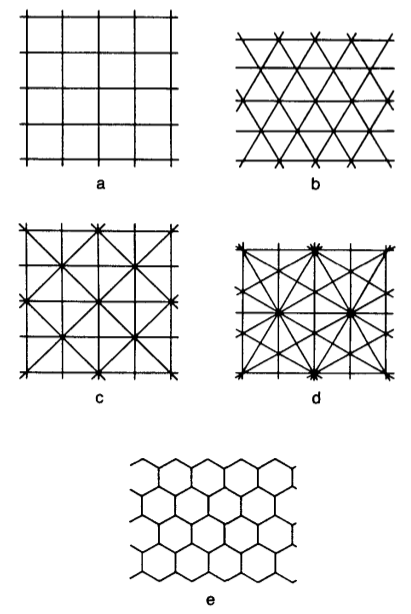
\includegraphics[width=0.5\textwidth]{figures/space_decompositions.png}
    \label{fig:space-decompositions}
    \caption{Sample tessellations: (a) $[4^4]$ square; (b) $[6^3]$ equilateral triangle; (c) $[4.8^2]$ isoceles triangle; (d) $[4.6.12]$ 30-60 right triangle; (e) $[3^6]$ hexagon~\cite[p 17]{Samet90spatialdata}.}
  \end{center}
\end{figure}

The simplest polygonal space decomposition method is based on squares. It is directly related to the Morton and Peano-Hilbert space order methods as described in the previous chapter \ref{chapter:space-order}. Both orders work in a hierarchical manner and visit entire sub-quadrants first before continuing further. This is why they are predestined to decomposing space into squares as indicated in Figures~\ref{fig:space-orders}~and~\ref{fig:space-decompositions}.

\subsection{Quadtree}

Quadtrees are hierarchical data structures based on recursive decomposition of space. Their original motivation was to optimize storage by aggregating identical or similar values. Over time they have also been studied to optimize execution time of spatial application and have been established as a common practice for representing and storing spatial data. The resolution of a quadtree can be fixed or variable and directly relates to the number of decomposition times of the space where the data points live. A standardized implementation is the region quadtree which subdivides space into four equal-sized quadrants.

\begin{figure}[h]
  \begin{center}
    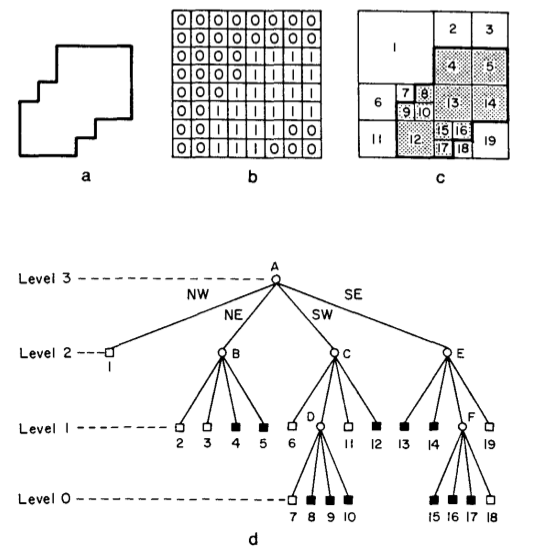
\includegraphics[width=0.7\textwidth]{figures/quadtree.png}
    \label{fig:space-decompositions}
    \caption{An example of (a) a region, (b) its binary array, (c) its maximal blocks (blocks in the region are shaded), and (d) the corresponding quadtree~\cite[p 3]{Samet90spatialdata}.}
  \end{center}
\end{figure}

Quadtrees can be constructed in different ways. A top-down approach implements the Morton order which maps the multidimensional data to one dimension and has been introduced in chapter~\ref{chapter:space-order}. Also note that the term quadtree has taken various meanings: actually it is a trie (or digital tree) structure because each data key is a sequence of characters. ``A node at depth $i$ in the trie represents an $M$-way branch depending on the $i$-th character'' \cite{Samet90spatialdata}.

\subsection{Geohash}
\label{chapter:geohash}

Geohash is a latitude/longitude geocode system based on the Morton order, described in \ref{chapter:space-order}. It encodes geographic point coordinates into string identifiers that reflect a hierarchical spatial structure. Its gradual precision degradation property means that if two geohashes share a common prefix, their closeness is described by the length of the shared prefix~\cite{wiki:geohash, Smiley11geohash}.

Originally, the geohash encoding algorithm has been developed and put into the public domain by Gustavo Niemeyer when creating the web service \href{http://geohash.org}{geohash.org}. The service allows to encode spatial coordinates into unique string identifiers and vice versa~\cite{wiki:geohash}. Amongst other applications, it has also been incorporated into geospatial search plugins of the Apache Solr search platform~\cite{Smiley11geohash} and leveraged for real-time, location-aware collaborative filtering of web content by HP Labs~\cite{Sand11geohashapp}.

A geohash is constructed by interleaving the bits of the latitude and longitude values and converting them into a string of characters using a Base 32 encoding. As every Base 32 symbol is represented by an uneven number of 5 bits, the resulting  space decomposition is a rectangular grid formed by $4 \times 8$ or $8 \times 4$ cells. The orientation of the resulting rectangles alternates between vertical for characters of an odd index and horizontal for such characters that are positioned at an even index within the geohash. Figure \ref{fig:geohash} illustrates how the first character of a geohash string splits the projected earth into an $8 \times 4$ grid of horizontally aligned rectangles~\cite{wiki:geohash, Smiley11geohash}.

\begin{figure}[h]
  \begin{center}
    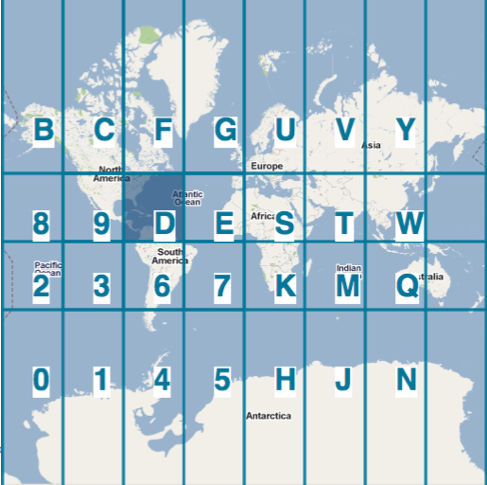
\includegraphics[width=0.7\textwidth]{figures/geohash_example.png}
    \label{fig:geohash}
    \caption{Space decomposition of the geohash algorithm on the first level~\cite{Smiley11geohash}.}
  \end{center}
\end{figure}

The fact that points with a common prefix are near each other must not be confused with the converse. Due to the nature of the morton order, edge cases exist. Two points may be very close to each other, without sharing an equally long prefix. Figure \ref{fig:geohash-edge} illustrates an example of two closely positioned points being located within different geohashes. The first point being at the very lower end of the ``DRT'' geohash and the second point positioned closely at the upper end of the ``DRM'' geohash. 

\begin{figure}[h]
  \begin{center}
    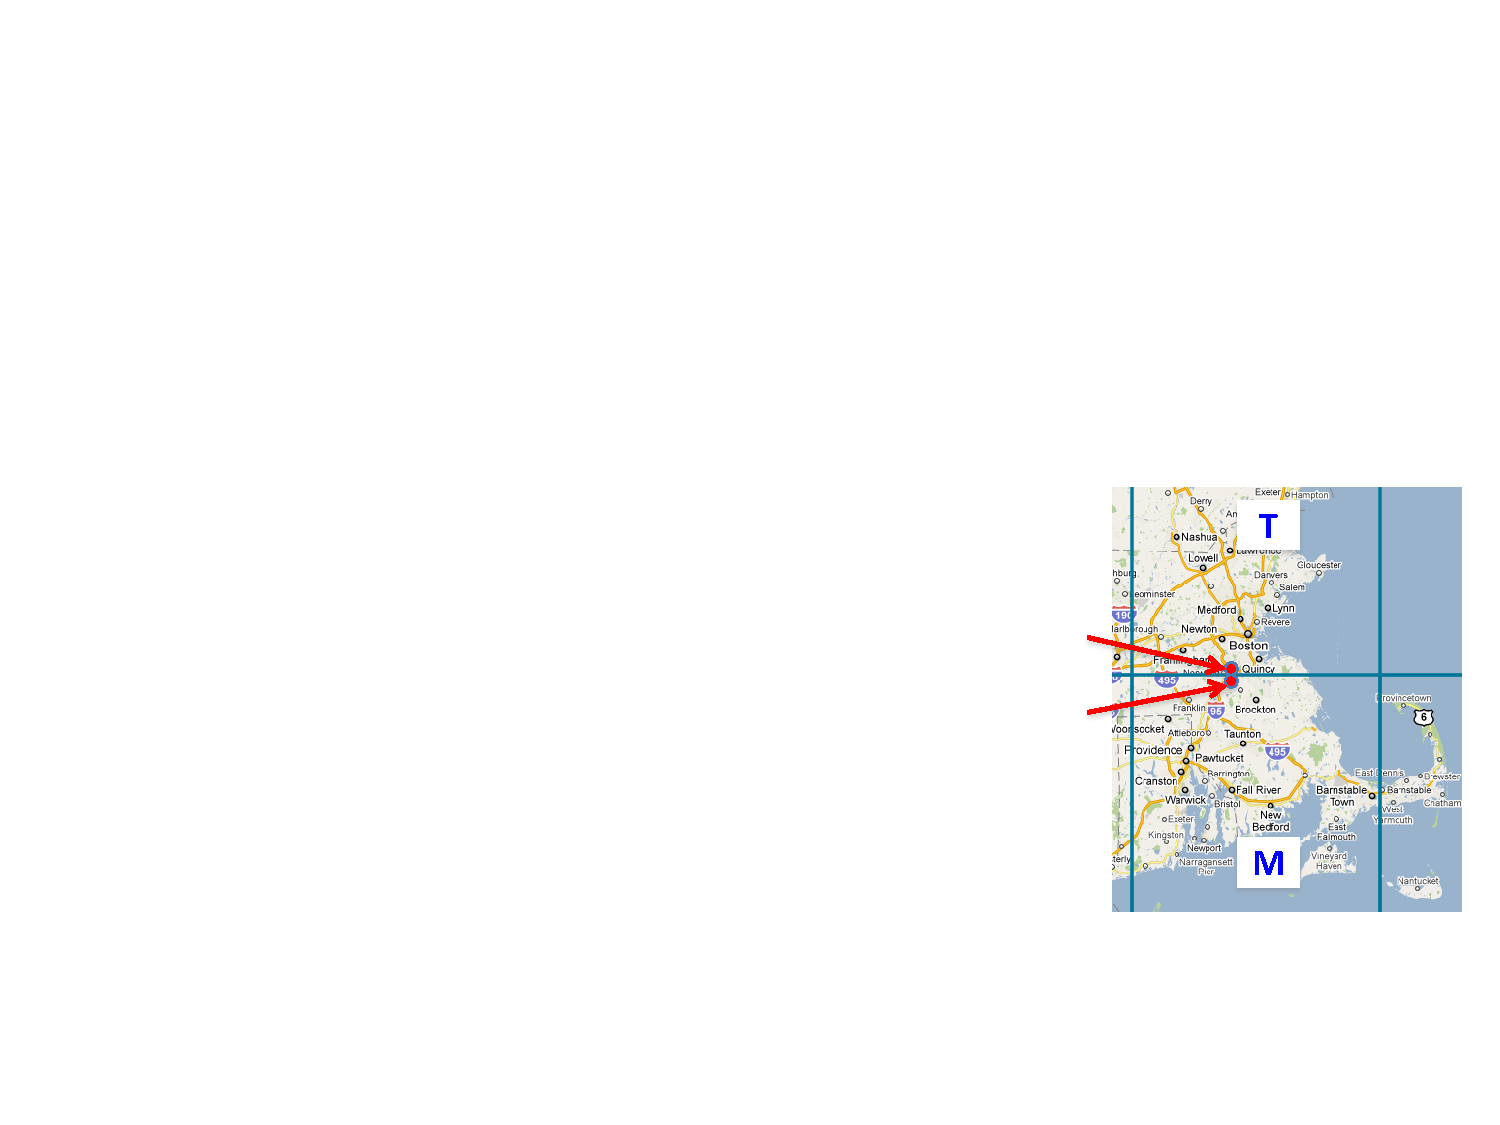
\includegraphics[width=0.7\textwidth]{figures/geohash_edges.pdf}
    \label{fig:geohash-edge}
    \caption{Space decomposition of the geohash algorithm on the first level~\cite{Smiley11geohash}.}
  \end{center}
\end{figure}



























